\chapter{NLP with DL}\label{sec:nlp}

\chapternote{Natural Language Processing with Deep Learning}{Stanford CS224n Winter 2019}

\begin{learningobjectives}
	\item Word Vector
	\item Calculus Review
	\item RNN \& Language Model
	\item Seq2Seq \& Attention
	\item ConvNet for NLP
	\item Transformer
\end{learningobjectives}

\dependencies{Machine Learning Basic}


\section{Word Vector}

Arguably the most simple word vector, i.e., \concept{one-hot vector}: an $\R^{|V| * 1}$ vector with one $1$ and the rest $0$s.
Note that these one-hot vectors are \concept{orthogonal} (i.e., no similarity/relastionship) and $V$ is a very big vocabulary ($\sim 500k$ words for english).

\sidenotedcmmc{In traditional NLP (before 2013), words are regarded as discrete symbols (\concept{localist} representation) and cannot capture similarity. One-hot vector is an example.}

Another idea: \concept{distributional representation} in modern statistical NLP. A word's meaning is given by the words that frequently appear close-by.
Using some $N$-dim ($N \ll |V|$) space is sufficient to encode all semantics of our language into a dense vector.
Once we get the word embedding matrix where each column is a word vector, we can query the word vector from one-hot representation by treating it as \concept{lookup table} instead of using matrix product.

\Figure{word_analogy}{An example of word analogy of man:woman :: king:?}

To evaluate word vectors, there are two fold: \emph{intrinsic} (directly used, e.g. word analogies/similarity) and \emph{extrinsic} (indirectly used in real task, e.g. Q\&A).
Word vector analygies for  $a:b :: c:\textcolor{red}{d}$ is calculated by cosine similarity as example shown in Fig.~\ref{fig:word_analogy}:

\begin{equation}
d = \arg \max_i \frac{(x_b - x_a + x_c)^\top x_i}{\lVert x_b - x_a + x_c \rVert}
\end{equation}

If we have hundreds of millions of words, it's okay to start the vectors \emph{randomly}.
If there is a \emph{small} ($\le 100,000$) training data set, it's best to just treat the pre-trained word vectors as \emph{fixed}.
In the other hand, if there is a large dataset, then we can gain by \concept{fine tuning} of the word vectors.

\subsection{Word2vec}

Two families of models: \concept{Skip-gram} and \concept{Continuous Bag of Words}.

Idea of \concept{Skip-gram} (predicting context words by a given center word) in  Word2vec\mycite{word2vec}:

\begin{itemize}
	\item a large corpus of text $T$ with a vocabulary $V$
	\item every word is represented by a vector $w \in \mathbb{R}^d$ and start off as a random vector
	\item use the (cosine) similarity of the word vectors for $c$ (center word) and $o$ (context/outside word) to calculate the probability of $o$ given $c$: $p(w_o | w_c)$
	\item adjusting the word vectors to maximize the probability
\end{itemize}

\sidenotedcmmc{Why we use two vectors per word? Make it simpler to calculate the gradient of loss function. Because the center word would be one of the choices for the context word and thus squared terms are imported. Average both vectors at the end is the final word vector.}

The conditional probability is calculated by the \concept{softmax} (normalize to probability distribution) of \concept{cosine} similarity (review dot product: $\bm{a} \cdot \bm{b} = |\bm{a}||\bm{b}| \cos\left<\bm{a}, \bm{b}\right>$).
Note that the visualization of word vectos utilizes 2D projection (e.g. PCA) that will loss huge information.

\begin{equation}
p(w_o | w_c) = \frac{\exp(u_o^\top v_c)}{\sum_{w \in V}(u_w^\top v_c)}
\end{equation}
where $v_c$ denotes the center word vector of $w$ when $w$ is used as a center word in the formula, and $u_w$ denotes the context word vector of $w$ as the similar way.
A demo of the window size and conditional probability is shown in Fig.~\ref{fig:word2vec:window_cond}.

\MoveNextFigure{+5cm}
\Figure{word2vec:window_cond}{A demo of the window size and $p(w_o | w_c)$}


The objective function (a.k.a loss or cost function) is given by the (average) negative log likelihood (abbr. \concept{NLL}).
The parameters of the model are adjusted by minimizing the loss function $J(\theta)$ or maximizing the likelihood.
This is, give a high probability estimate to those words that occur in the context and low probability to those don't typically occur in the context.


\begin{align}
	\arg\max_\theta L(\theta) &= \prod_{c=1}^{T} p(w_{c-m}, \cdots, w_{c-1}, w_{c+1}, \cdots, w_{c+m} | w_c; \theta) \nonumber \\
	&= \prod_{c=1}^{T} \prod_{\substack{-m \le j \le m \\ o = j + c \\ o \ne c}} p(w_o | w_c; \theta) \nonumber \\
	&\Downarrow \nonumber \\
	\arg\min_\theta -\frac{1}{T} \log L(\theta) &= -\frac{1}{T} \sum_{c=1}^{T} \sum_{ \substack{-m \le j \le m \\ o=j+c \\ o \ne c}} \log p(w_o | w_c; \theta) \nonumber \\
	&= -\frac{1}{T} \sum_{c=1}^{T} \sum_{ \substack{-m \le j \le m \\ o=j+c \\ o \ne c}} \left( u_o^\top v_c - \log \sum_{w \in V} \exp(u_w^\top v_c)\right) 
	\label{eq:word2vec_loss}
\end{align}
where $m$ is the window size, $\theta \in \mathbb{R}^{2d|V|}$ represents all model parameters.
And we assume that $p(\cdot | w_c)$ are \concept{i.i.d}.

\sidenotedcmmc{The properties of $\log$ and $\arg \max$ ($\arg \min$) used in Eq.~\ref{eq:word2vec_loss} are VERY useful. $\exp(\cdot)$ ensures anything positive.}

We use \concept{gradient descent} (i.e. averaged gradient of all samples/windows) to optimize the loss function.
Note that stochastic (one sample/window with noisy estimates of the gradients) or mini-batch (a subset of samples/windows with size powered of $2$ such as $64$) gradient descent methods are useful to prevent overfitting and train for large dataset.
Calculating the gradient of the loss function is trivial:

\begin{equation}
\begin{split}
\frac{\partial J}{\partial v_c} &= -\frac{1}{T} \sum_{c=1}^{T} \sum_{ \substack{-m \le j \le m \\ o=j+c \\ o \ne c}} \left(u_o - \sum_{x \in V} \frac{\exp(u_x^\top v_c) u_x}{\sum_w \exp(u_w^\top v_c)}\right) \\
&= -\frac{1}{T} \sum_{c=1}^{T} \sum_{ \substack{-m \le j \le m \\ o=j+c \\ o \ne c}} \left(u_o - \sum_{x \in V} p(w_x | w_c) \cdot u_x \right)
\end{split}
\end{equation}

\begin{equation}
\frac{\partial J}{\partial u_o} = -\frac{1}{T} \sum_{c=1}^{T} \sum_{ \substack{-m \le j \le m \\ o=j+c \\ o \ne c}} \left(v_c - p(w_o | w_c)\right)
\end{equation}

Iteratively update equation (na\"ive version) is given by:

\begin{equation}
\theta^{new} = \theta^{old} - \alpha \nabla_\theta J(\theta)
\end{equation}
where $\alpha$ is the learning size (step size) such as $10^{-3}$.

Note that the summation over $|V|$ ($\sum_{x \in V}$) is very expensive to compute!
For every training step, instead of looping over the entire vocabulary, we can just sample several negative examples!
\concept{negative sampling}: train binary logistic regression instead.
$p(D=1|w_o,w_c)$ denotes the probability when $(w_o,w_c)$ came from the same window pf the corpus data, and $p(D=0|w_o,\tilde{w}_o)$ is the probability given $(w_o,\tilde{w}_o)$ did not come from the same window (i.e. noisy/invalid pair).
Randomly sample a bunch of noise words from the \concept{unigram distribution} raised to the power of $3/4$: $p(w) = \nicefrac{U(w)^{3/4}}{Z}$, where $U(w)$ is the counts for every unique words (i.e. unigram) and $Z$ is the nomalization term.

To avoid high frequence effect of words such as \concept{of} and \concept{the}, one simple way is just lop off the first biggest component in the word vector.
The unigram with power of $3/4$ in word2vec is also a trick to handle the effect, where it decrease how often you sample very common words and increase how often you sample rare words.

The objective function is also come from NLL: 

\begin{equation}
J(\theta) = - \frac{1}{T} \sum_{c=1}^T \sum_{ \substack{-m \le j \le m \\ o=j+c \\ o \ne c}} \left( \log \sigma \left( u_o^\top v_c \right) + \sum_{j \sim p(w)} \left[ \log \sigma \left(-u_j^\top v_c\right) \right] \right)
\end{equation}
where \concept{sigmoid} function is $\sigma(x) = \frac{1}{1 + e^{-x}}$ which can be seen as the 1D (binary) version of softmax and used to output the probability, and $k$ is the number of negative samples such as $5$ and $15$.
Note that according to the symmetric property of sigmoid function we get: $P(D=0|\tilde{w}_j,w_c) = 1 - P(D=1|\tilde{w}_j,w_c) = \sigma \left(-u_j^\top v_c\right)$.

\sidenotedcmmc{Although word2vec model is fairly simple and clean, there are actually many tricks which aren't particularly theoretical.}

\concept{Continuous Bag of Words} (CBOW): predict center word from (bag of) context words.
Similar to Skip-gram, the objective function is formulated as:

\begin{align}
J &= -\frac{1}{T} \sum_{c=1}^{T} \log P (w_c | w_{c-m}, \cdots, w_{c-1}, w_{c+1}, \cdots, w_{c+m}) \\
&= -\frac{1}{T} \sum_{c=1}^{T} \log p (v_c | \hat{u}) \\
&= -\frac{1}{T} \sum_{c=1}^{T} \log \mathop{\textup{softmax}}\limits_{c}(v_c^\top \hat{u}) \\
&= -\frac{1}{T} \sum_{c=1}^{T} (v_c^\top \hat{u} - \log \sum_{j=1}^{|V|} \exp (v_j^\top \hat{u}))
\end{align}
where $\hat{u} = \frac{1}{2m} \sum_{ \substack{-m \le j \le m \\ o=j+c \\ o \ne c}} u_o$


Although word2vec can capture complex patterns beyond word similarity, it has inefficient usage of statistics (i.e. rely on sampling rather than directly use counts of words).

\subsection{HW1}

A simple intro to co-occurrence matrix, SVD, cosine similarity, and some applications (e.g. word analogy) of word2vec.

\subsection{GloVe}
\Figure{cooccurrence_matrix}{An example of co-occurrence matrix with window size of $1$}

Co-occurrence matrix $X \in \mathbb{R}^{|V| * |V|}$ with window size $k$.
Fig.~\ref{fig:cooccurrence_matrix} shows an example.
Note that such matrix is extremely sparse and very high dimensional, and the dimensions of the matrix change very often as new words are added very frequently and corpus changes in size.
We can perform SVD on $X$ to reduce the dimensionality to $25 \sim 1000$-dim.
In addition, there are some hacks to $X$ that transform the raw count introduced by \mycite{rohde2005_hacks}: (1) set upper bound (e.g. $100$) or just ignore them all for the counts of too frequent words, (2) ramped windows that count closer words more. (3) use Pearson correlations instead of counts.
Note that they made some interesting observation in their word vector that the verb (e.g. swim) and the corresponding doer (e.g. swimmer) pairs are roughly \emph{linear components} (e.g. $\bm{v}_{swimmer} - \bm{v}_{swim} = k (\bm{v}_{driver} - \bm{v}_{drive})$).

\tododcmmc{SVD}

Although the aforementioned conventional method has disproportionate importance given to large counts and mainly only capture word similarity, it enjoys the fast training and efficient usage of statistics.
GloVe (\textbf{Glo}bal \textbf{Ve}ctor) \mycite{GloVe} combines the advantages from both of this conventional method (global count matrix factorization) and the DL-based methods (local context window methods) such as word2vec.
It captures global corpus statistics directly.

\Figure{ratio_cooccurrence}{An example of the conditional probabilities and their ratio in GloVe paper.}

Some notations: $X_{ij}$ tabulate the number of times word $j$ occurs in the context of word $i$, $X_i = \sum_{k} X_ik$ is the number of times any word appears in the context of word $i$ i.e., the nomalization denominator.
$P_{ij} = P(j|i) = \nicefrac{X_{ij}}{X_i}$ is the probability that word $j$ appear in the context of word $i$.
The crucial insight is that the \emph{ratios} of co-occurrence probabilities as shown in Fig.~\ref{fig:ratio_cooccurrence} to encode meaning components.
We'd like to leverage the word vectors $w_i, w_j, \tilde{w}_k$ to represent such ratio: $F(w_i, w_j, \tilde{w}_k) = \nicefrac{P_{ik}}{P{jk}}$, where $\tilde{w}$ is a seperate \emph{context} word vector for various \emph{probe words} $k$, instead of the word vector $w$ (similar to center word vector in skip-gram).

We can select a unique choice of $F$ by enforcing a few desiderata (i.e. restrictions).
To fit the demand of the \emph{linear components} and the output \emph{scalar} value, in addition to the \emph{homomorphism}
between the groups $(\mathbb{R}, -)$ and $(\mathbb{R}^+, \div)$ (i.e., $F(i,j) = \nicefrac{P_{ik}}{P{jk}} = \nicefrac{1}{F(j,i)} = \nicefrac{P_{jk}}{P{ik}}$), we can derivate that $F(w_i, w_j, \tilde{w}_k) = F\left((w_i - w_j)^\top \tilde{w}_k\right) = \nicefrac{F(w_i^\top \tilde{w}_k)}{F(w_j^\top \tilde{w}_k)} = \nicefrac{P_{ik}}{P_{jk}}$.
Therefore, $F=\exp, w_i^\top \tilde{w}_k = \log(P_{ik}) = \log (X_{ik}) - \log (X_i)$.
Note that the symmetry property of co-occurrence: $X_{ik} = X_{ki}$.
We add two biases to restore the symmetry: $w_i^\top \tilde{w}_k + b_i + \tilde{b}_k = \log (X_{ik})$, where we can analogy that $b_i + \tilde{b}_j = \log X_{i}$.

More details, the relationship to the "global skip-gram" and the complexity refer to the original GloVe paper~\mycite{GloVe}.

\sidenotedcmmc{To handle the ill-defined $\log$ function when its argument be $0$ (its common that $X_{ij}=0$), the authors use the factorized log: $\log(X_{ik}) \rightarrow \log (1+X_{ik})$.}

\begin{align}
w_i \cdot w_j &= \log P(i|j) \\
w_x \cdot (w_a - w_b) &= \log \frac{P(x|a)}{P(x|b)}
\end{align}

Therefore, the ratios of co-occurrence probabilities is the \concept{log-bilinear model with vector differences}.
The final objective function is \emph{weighted} \concept{least squares} (MSE) for this regression problem.

\begin{equation}
	J = \sum_{i,j=1}^V f(X_{ij})\left(w_i^\top \tilde{w}_j + b_i + \tilde{b}_j - 
	log X_{ij}\right)
\end{equation}
where weighted function (is also a hyperparamter) is:

\begin{equation}
f(x) =
\begin{cases}
	\left(\frac{x}{x_{max}}\right)^\alpha & \text{if } x < x_{max} \\
	1 & \text{otherwise}
\end{cases}
\end{equation}
where $x_{max} = 100, \alpha = \nicefrac{3}{4}$ (\emph{empirical} value). 

\subsection{Word sense ambiguity}
Because most words have lots of meanings.
One crude way \mycite{huang-etal-2012-improving} is to cluster word windows around words, retrain with each
word assigned to multiple different clusters $\textsf{bank}_1$, $\textsf{bank}_2$, etc.
Another method \mycite{TACL_word_senses} is weighted sum of different senses of a word reside in a linear superposition, e.g.:

\begin{equation}
v_{\text{pike}} = \alpha_1 v_{\text{pike}_1} + \alpha_2 v_{\text{pike}_2} + \alpha_3 v_{\text{pike}_3}
\end{equation}
where $\alpha_i = \frac{f_i}{\sum_{j=1}^3 f_j}$ for frequency $f$.

The result is counterintuitive very well, because of the idea from \emph{sparse} coding you can actually separate out the senses.

\section{Math Backgrounds}
For \concept{multi-class classification} problem, \concept{NLL} (negative likelihood loss) is the objective function of \concept{Maximum Likelihood Estimate} (abbr, MLE):

\begin{equation}
J(\bm{\theta}) = - \sum_i \log p(y = y^{true}_i | \bm{x}_i; \bm{\theta})
\end{equation}

\concept{cross entropy} (distance measure) between (discrete) distribution $p$ and $q$ is more convenient way:

\begin{equation}
H(p, q) = - \sum_{c=1}^C p(c) \log q(c)
\end{equation}

However, in the multi-class (with single label) setting, the p(c) is the \concept{ground truth distribution} which has the \emph{one-hot} style (\concept{empirical distribution}), i.e. $p = [0, \cdots, 0, 1, 0, \cdots, 0]$ where $1$ at the right class and $0$ everywhere else.
Therefore, the \concept{cross entropy} in the multi-class classification is \emph{equal} to the NLL.

A simple $k$-class model example is \concept{dense layer} with \emph{softmax}:

\begin{equation}
	p(y|\bm{x}; \bm{\theta}) = softmax(\bm{W}_2 f(\bm{W}_1 \bm{x} + \bm{b}))
\end{equation}
where $\bm{\theta} = [\bm{W}_1, \bm{b}, \bm{W}_2]^\top $ are the parameters, $\bm{x} \in \mathbb{R}^m, \bm{W}_1 \in \mathbb{R}^{n * m}, \bm{b} \in \mathbb{R}^n, \bm{W}_2 \in \mathbb{R}^{k * n}$, $f(\cdot)$ is a kind of simple activate (non-linear) function to provide non-linearity, such as $ReLU(x) = max(0, x)$.
The visualization of neural network refer to \sidenote{ ConvNetJS: \url{https://cs.stanford.edu/people/karpathy/convnetjs/demo/classify2d.html}}.

The \concept{Jacobian Matrix} (generalization of the gradient) of function $\bm{f}(\bm{x}): \mathbb{R}^n \rightarrow \mathbb{R}^m$ is a $m \times n$ matrix: $\left(\frac{\partial \bm{f}}{\partial \bm{x}}\right)_{ij} = \frac{\partial f_i}{x_j}$.

Supposed that we have a function $\bm{g}(\bm{f}(x)), \bm{f}: \mathbb{R} \rightarrow \mathbb{R}^2, \bm{g}: \mathbb{R}^2 \rightarrow \mathbb{R}^2$, we can compute the partial derivative of $\bm{g}$ w.r.t $x$ by \concept{chain rule}:

\begin{equation}
	\frac{\partial \bm{g}}{\partial x} = \begin{bmatrix}
	\frac{\partial g_1}{\partial f_1} \frac{\partial f_1}{x} + \frac{\partial g_1}{\partial f_2} \frac{\partial f_2}{x}\\
	\frac{\partial g_2}{\partial f_1} \frac{\partial f_1}{x} + \frac{\partial g_2}{\partial f_2} \frac{\partial f_2}{x}
	\end{bmatrix}
\end{equation}

\sidenotedcmmc{$\frac{d g_1}{d \bm{y}} = \frac{\partial g_1}{y_1} + \frac{\partial g_2}{y_2}$ is the relationship of the full differential and the partial differential.}

It is the same as multiplying the two Jacobians:

\begin{equation}
\frac{\partial \bm{g}}{\partial x} = \frac{\partial \bm{g}}{\partial \bm{f}} \frac{\partial \bm{f}}{\partial x} = \begin{bmatrix}
\frac{\partial g_1}{\partial f_1} & \frac{\partial g_1}{\partial f_2} \\
\frac{\partial g_2}{\partial f_1} & \frac{\partial g_2}{\partial f_2}
\end{bmatrix} \begin{bmatrix}
\frac{\partial f_1}{\partial x} \\
\frac{\partial f_2}{\partial x}
\end{bmatrix}
\end{equation}

There are some useful identities:

\begin{itemize}
	\item $\frac{\partial \bm{x}}{\partial \bm{x}} = \bm{I}$
	\item $\frac{\partial \bm{Wx}}{\partial \bm{x}} = \bm{W}, \frac{\partial \bm{u}^\top \bm{x}}{\partial \bm{x}} = \bm{u}^\top$
	\item $\frac{\partial \bm{x^\top W}}{\partial \bm{x}} = \bm{W^\top}$
	\item For elemenwise function $\bm{f}(\bm{x})$: $\frac{\partial \bm{f}}{\partial \bm{x}} = \texttt{diag}(\bm{f}^\prime(\bm{x}))$
	\item $\frac{\partial \bm{\theta}^\top (\bm{W} \cdot \bm{h})}{\partial \bm{W}} = \bm{\theta} \bm{h}^\top$ where $\bm{\theta} \in \mathbb{R}^{D_\theta * 1}, \bm{W} \in \mathbb{R}^{D_\theta * D_h}, \bm{h} \in \mathbb{R}^{D_h * 1}$
	\item For cross entropy loss: $J(\bm{h}) = - \bm{y}^\top \log (\hat{\bm{y}}) = - \bm{y}^\top \log \texttt{softmax}(\bm{h})$ ($\bm{y}$ is one-hot vector) is: $\frac{\partial J}{\partial \bm{h}} = (\hat{\bm{y}} - \bm{y})^\top$
\end{itemize}

We can use \concept{backward propagation} (reversed of the \emph{topological sort}) and \emph{re-use} intermediate nodes to reduce complexity in the \emph{computation graph}.

Other machine learning basic concepts are: \concept{regularization} (e.g. L2) to prevent \concept{overfitting}, vectorization to parallelization, (non-linear) \concept{activation function} (e.g. sigmoid, tanh, (leaky) ReLU), parameter initialization (e.g. Xavier), \concept{Optimizer} (e.g. RMSprop, Adam), learning rate.

\subsection{Data Preprocessing}
\Figure{mean_subtraction}{An exmaple of mean subtration.}
\Figure{normalization}{An example of normalization.}

\begin{itemize}
	\item \textbf{Mean Subtraction (Shifting)}: Shifting all data so that they have zero mean as shown in Fig.~\ref{fig:mean_subtraction}. Formally, $\bm{x}^{(i)} \leftarrow \bm{x}^{(i)} - \mathbb{E}[\bm{x}^{(i)}]$ for sample $i$, where $\mathbb{E}$ indicates mean.
	\item \textbf{Normalization (Scaling)}: Scale every input feature dimension to have
	similar ranges of magnitudes, as shown in Fig.~\ref{fig:normalization}. This is useful since input features are often measured in different "units", but we often want to initially consider all features as equally important. Formally, $x^{(i)}_{j} \leftarrow \frac{x^{(i)}_{j}}{\sigma_i (x^{(i)}_{j})}$ for feature $j$ in sample $i$ where $\sigma(\cdot)$ is the standard variance over $x^{(0)}_{j}, \cdots, x^{(N)}_{j}$.
	\item \textbf{Whitening}: Whitening converts the data to a have an identity covariance matrix - that is, features become uncorrelated and have a variance of $1$. In the specific, we can divide the principal components achieved from PCA by the square roots of their eigenvalues (singular value).
\end{itemize}

\subsection{Parameter Initialization}
	
If two hidden units have exactly the same bias and exactly the same incoming and outgoing weights (e.g. different channels for learning different features in the same convolutional layer), they will always get exactly the same gradient.
So we should initialize the weights to small random values.

A good starting strategy is to initialize the weights to small random numbers of \concept{normal distribution} with the mean around $0$.
Xavier et al. \mycite{Xavier} suggest that for sigmoid and tanh activation units, it's better for the weight matrix $W \in \mathbb{R}^{n^{(l+1)} * n^{(l)}}$ to be initialized randomly with a \concept{uniform distribution}:
\begin{equation}
W \sim U\left[- \sqrt{\frac{6}{n^{(l)} + n^{(l+1)}}}, \sqrt{\frac{6}{n^{(l)} + n^{(l+1)}}}\right]
\end{equation}
where $n^{(l)}, n^{(l+1)}$ are also called \textbf{fan-in} and \textbf{fan-out}.

\subsection{Optimizer}
To avoid a diverging loss (too large learning step) or unconverging (too small learning step), there are some learning strategies.

\concept{Annealing}: start off with a high learning rate to approach a minimum quickly, after several iterations, the learning rate is reduced in some way under a more fine-grained scope.
\begin{itemize}
	\item Exponential decay: $\alpha(t) = \alpha_0 e^{-kt}$ where $\alpha_0$ is initial learning rate.
	\item Decrease over time: $\alpha(t) = \nicefrac{(\alpha_0 \tau)}{\max(t, \tau)}$ where $\tau$ denotes the time at which the learning rate should start reducing.
\end{itemize}

\Figure{momentum}{A picture of momentum.}

\concept{Momentum} (a picture of it can be seen in Fig.\ref{fig:momentum}) based methods:
\begin{itemize}
	\item AdaGrad: $\bm{m} \leftarrow \bm{m} + \left(\nabla_{\bm{\theta}} J (\bm{\theta})\right)^2, \bm{\theta} \leftarrow \bm{\theta} - \alpha \nabla_{\bm{\theta}} J (\bm{\theta}) \odot \left(\sqrt{\bm{m}} + \epsilon\right)^{-1}$ where $\odot, (\cdot)^{-1}, (\cdot)^{2}, \sqrt{\cdot}$ are all element-wise operators, and $\epsilon$ is a very small value such as $10^{-8}$ to prevent \concept{arithmetic underflow}.
	It leads to that parameters that have not been updated much in the past are likelier to have higher learning rates now.
	\item RMSprop: $\bm{m} \leftarrow \beta \bm{m} + (1-\beta) \left(\nabla_{\bm{\theta}} J (\bm{\theta})\right)^2, \bm{\theta} \leftarrow \bm{\theta} - \alpha \nabla_{\bm{\theta}} J (\bm{\theta}) \odot \left(\sqrt{\bm{m}} + \epsilon\right)^{-1}$ where $\beta$ is the decay rate with default value $0.9$. Unlike AdaGrad, its updates do not become monotonically smaller.
	\item Adam\mycite{Adam}: $\bm{m} \leftarrow \beta_1 \bm{m} + (1-\beta_1) \nabla_{\bm{\theta}} J (\bm{\theta}), \bm{v} \leftarrow \beta_2 \bm{v} + (1-\beta_2) \left(\nabla_{\bm{\theta}} J (\bm{\theta})\right)^2, \hat{\bm{m}} = \bm{m} / (1 - \beta_1^t), \hat{\bm{v}} = \bm{v} / (1 - \beta_2^t), \bm{\theta} \leftarrow \bm{\theta} - \alpha \hat{\bm{m}} /  \left(\sqrt{\hat{\bm{v}}} + \epsilon\right)^{-1}$, where $/$ is also a element-wise operator, hyperparameters $\beta_1 = 0.9, \beta_2 = 0.999 \in [0, 1)$. $\hat{\bm{m}}, \hat{\bm{v}}$ are the bias-corrected $\bm{m}, \bm{v}$, and they indicate a rolling average
	of the gradients and a rolling average of the magnitudes of the gradients, respectively. In adition, $\bm{m}, \bm{v}$ are all initialized to $\bm{0}$ Adam is like a combination of RMSProp and momentum.
\end{itemize}

\sidenotedcmmc{For the implementation of momentum such as RMSprop, there is a interesting small trick: use $\bm{m} = \bm{m} - (1-\beta)(\bm{m} - \left(\nabla_{\bm{\theta}} J (\bm{\theta})\right)^2)$ instead of $\bm{m} = \beta \bm{m} + (1-\beta) \left(\nabla_{\bm{\theta}} J (\bm{\theta})\right)^2$. In such way, we need calculate only one multiplication, compared with original two multiplications.}

\subsection{Regularization}
\textbf{1. Dropout}

During training, \concept{dropout} \mycite{dropout} randomly disables units in the hidden layer by a mask vector drawn from Bernoulli distribution where each entry is $0$ with probability $p_{\text{drop}}$ and $1$ with probability ($1 − p_{\text{drop}}$):
\begin{equation}
\text{Dropout Layer: } \textcolor{red}{d_i \sim \text{Bernoulli}(1 - p_{\text{drop}}), \hat{\bm{h}}^{(t)} = } \textcolor{blue}{\frac{1}{1-p_{\text{drop}}}} \textcolor{red}{\bm{d} \odot \bm{h}^{(t)}}
\end{equation}
where $\odot$ is element-wise product, $\bm{d} \in \{0, 1\}^{D_h}, \bm{h}^{(t)} \in \mathbb{R}^{D_h}$.

If the expected output of a neuron during testing if far different as it was during training, the magnitude of the outputs could be radically different, and the behavior of the network is no longer well-defined.
Therefore, all the parameters should divided by retain rate $1-p$ (blue part in above formula), so that $\mathbb{E}_{P_{\text{drop}}} [\bm{h}_{\text{drop}}]_i = h_i$.
If we do not such correction in training, we should multiply $1-p$ to all related parameters.

If we use dropout in testing, the result is \emph{unstable} (vary from every testing) because of the
dropout is drawn from Bernoulli distribution.
Therefore, we should apply dropout only during training but not during evaluation or testing.

\textbf{2. Batch Normalization}

Although \concept{batch nomalization} \mycite{BatchNorm} is like nomalization used in data preprocessing with $N$ be the mini-batch size instead of the dataset size, it is inserted between hidden layers to normalize the output of last layer.
It leads to achieve the fixed distributions of inputs that would remove the ill effects of the internal covariate shift.
\emph{Internal Covariate Shift} is defined as the change in the distribution of network activations due to the change in network parameters during training.

The batch normalization in training is defined as follows:
\begin{equation}
\text{BN}(h_i) = \gamma \frac{h_i - \mu_{\mathcal{B}}}{\sqrt{\sigma_{\mathcal{B}}^2 + \epsilon}} + \beta
\end{equation}
where $\gamma, \beta$ are \concept{trainable parameters}, $\mu_{\mathcal{B}}, \sigma_{\mathcal{B}}^2$ are the mean and variance over the mini-batch as the way of normalization for data preprocessing.
Since the mean subtraction will \emph{ignore} the learned bias which may useful to the model.
The trainable $\gamma$ and $\beta$ are used to corrected them and make the BN layer trainable.
Them ensure that the batch normalization inserted in the network can represent the identity transform.

However, when testing, we cannot use mini-batch in most time.
We instead feed one sample into the model.
Therefore, we leverage $m$ training mini-batches to perform \concept{unbiased estimates} of them:
\begin{align}
&\mathbb{E}[h_i] \leftarrow \mathbb{E}_{\mathcal{B}}[\mu_{\mathcal{B}}] \nonumber \\
&\texttt{Var}[h_i] \leftarrow \frac{m}{m-1} \mathbb{E}_{\mathcal{B}}[\sigma_{\mathcal{B}}^2] \nonumber
\end{align}

Note that in many implementations, the above estimation is replaced with the way like the momentum used in RMSprop.
More details refer to the source code, e.g. Keras.

\subsection{Practice: Named Entity Recognition}
To find and classify words as entities (e.g. location, or organization) in text.
One simple idea is that train softmax classifier to classify a center word by taking
\emph{concatenation} of word vectors surrounding it in a window (\emph{word window}) \mycite{NER_ICML}.
To perform NER of localtion, we need (unnormalized) score for each window, and make \emph{true window}’s (i.e. location in the center) score larger and other \emph{corrupt window}’s score lower.
The model is formulated as:

\begin{equation}
s = \bm{W}_2 f(\bm{W}_1 \bm{x} + \bm{b})
\end{equation}


The objective function (\emph{max-margin loss}) is:

\begin{equation}
J = max(0, s_c - (s - 1))
\end{equation}
where $s$ and $s_c$ is the score of true window and corrupt window.
It ensure each window with an NER location at its center should have a score $+1$ higher than any window without a location at its center.

\subsection{HW2}

Gradient calculation and implementation of word2vec.

\textbf{1. Written: Understanding word2vec}
\begin{align*}
	&(a) \ \hat{y}_o = P(O = o | C = c) \\
	&(b) \ \frac{\partial J}{\partial \bm{v}_c} = (\hat{\bm{y}} - \bm{y})^\top \bm{U}^\top \\
	&(c) \ \frac{\partial J}{\partial \bm{U}} = \bm{v}_c (\hat{\bm{y}} - \bm{y})^\top \\
	&(d) \ \sigma (\bm{x}) = \frac{1}{1 + \exp (- \bm{x})}, \frac{d \sigma (\bm{x})}{\bm{x}} = \texttt{diag} (\sigma (x_i) (1 - \sigma (x_i))) \\
	&(e) \ \frac{\partial J}{\partial \bm{v}_c} = \sum_k \sigma (\bm{u}_k^\top \bm{v}_c) \bm{u}_k^\top - (1 - \sigma (\bm{u}_o^\top \bm{v}_c)) \bm{u}_o^\top \\
	& \ \frac{\partial J}{\partial \bm{u}_o} = (\sigma (\bm{u}_o^\top \bm{v}_c) - 1) \bm{v}_c^\top \\
	& \ \frac{\partial J}{\partial \bm{u}_k} = \sigma (\bm{u}_k^\top \bm{v}_c) \bm{v}_c^\top \\
	&(f) \ (i) \frac{\partial J}{\partial \bm{U}} = \sum_o \bm{v}_c (\hat{\bm{y}}_o - \bm{y}_o)^\top \\
	&(ii) \frac{\partial J}{\partial \bm{v}_c} = \sum_o (\hat{\bm{y}}_o - \bm{y}_o)^\top \bm{U}^\top \\
	&(iii) \frac{\partial J}{\partial \bm{v}_w} = \bm{0}
\end{align*}

\sidenotedcmmc{Use shape convention to check the result.}

\textbf{2 Coding: Implementing word2vec}

Note that $\bm{U}, \bm{V}$ in the handout are the matrices whose $i$-th column is the $n$-dimensional embedded vector for word $w_i$.
However, in the codes of HW2, all the centerWordVectors and outsideVectors are as rows.

\section{Dependency Parser}
Two views of linguistic structure: (1) constituency (i.e., phrase structure grammar, or context-free grammar) (2) Dependency structure.
Dependence parse trees (single root with optional fake root, acyclic) use binary asymmetric relations which depicted as typed arrows going from \emph{head} to \emph{dependent}.
Note that the natural language is ambiguity.

Basic transition-based dependency parser \mycite{nivre-2003-efficient} with stack $\sigma = [\text{ROOT}]$, buffer $\beta = w_1, \cdots, w_n$, set of dependency arcs $A = \emptyset$, and a set of actions (\emph{transitions}) based on the above $3$-tuple:
\begin{align}
&\text{1. Shift: } \sigma , w_i | \beta, A \Rightarrow \sigma | w_i, \beta, A \nonumber \\
&\text{2. Left-Arc reduction: } \sigma | w_i | w_j, \beta, A \Rightarrow \sigma | w_j, \beta, A \cup \{r(w_j, w_i)\} \nonumber \\
&\text{3. Right-Arc reduction: } \sigma | w_i | w_j, \beta, A \Rightarrow \sigma | w_i, \beta, A \cup \{r(w_i, w_j)\} \nonumber
\end{align}
where $r(w_j, w_i)$ denotes $w_i$ is the dependency of $w_j$ (e.g. $\text{nsubj}(\text{ate} \rightarrow \text{I})$). The finish state is: $\sigma = [w], \beta = \emptyset$.
How to select (search) the best choice among the exponential size of different possible parse trees is the problem.
In 1960s, they use \emph{dynamic programming algorithms} ($\mathcal{O}(n^3)$).
In paper \mycite{nivre-2003-efficient}, the authors predict each action by a discriminative classifier (e.g. SVM classifier) which is more efficient but the accuracy is fractionally below the state-of-the-art.

\subsection{Neural Dependency Parsing}
Compared with traditional sparse feature-based discriminative dependency parsers, the work by \mycite{chen-manning-2014-fast} utilizes \concept{feedforward neural network model} with simple \concept{dense layers} and the softmax layer to predict each transition.
The input features with embedding dimension $d$ are:

\begin{enumerate}
	\item $x^{w} \in \mathbb{R}^{d * N_w}$: The top $3$ words on the stack and buffer $s_1, s_2, s_3, b_1, b_2, b_3$; the first and second leftmost / rightmost children of the top two words on the stack $lc_1(s_i), rc_1(s_i), lc_2(s_i), rc_2(s_i), i = 1, 2$; the
	leftmost of leftmost / rightmost of rightmost children of the top two words on the stack $lc_1(lc_1(s_i)), rc_1(rc_1(s_i)), i = 1, 2$; In total, $N_w = 18$.
	\item $x^{t} \in \mathbb{R}^{d * N_t}$: The corresponding POS (Part-of-speech, e.g. noun, verb, adjective) tags for $S_{word}$, $N_t = 18$.
	\item $x^{l} \in \mathbb{R}^{d * N_l}$:  The corresponding arc labels of words, excluding those $6$ words on the stack/buffer, $N_l = 12$.
\end{enumerate}

\sidenotedcmmc{Note that we use a special \textbf{NULL} token for non-existent elements: when the stack and buffer are empty or dependents have not been assigned yet.}

The predicted class is the one of transitions (i.e. shift, left/right arc reduction): $p = \texttt{softmax}(\bm{W}_2 f(\bm{W}_1^w \bm{x}^w + \bm{W}_1^t \bm{x}^t + \bm{W}_1^l \bm{x}^l + \bm{b}_1))$, where $f(\cdot)$ is the activation function (e.g. ReLU, or $x^3$).
The number of class is $3$ when untyped reductions or $T * 2 + 1$ when typed reductions (e.g. left-arc reduction with type \emph{nsubj}).

\subsection{HW3}
\textbf{1. Machine Learning \& Neural Networks}

\begin{enumerate}[label=(\alph*)]
	\item Adam
	\begin{enumerate}[label=(\roman*)]
		\item Because $\beta = 0.9$, most of the final gradients ($\bm{m}$) come from the past ($90\%$). Even if current gradients are varying much from previous, it only occupy $1 - \beta_1 = 0.1$ of the final gradients.
		\item Parameters that have not been updated much in the past are likelier to have higher learning rates.
	\end{enumerate}
	\item Dropout
	\begin{enumerate}[label=(\roman*)]
		\item If the expected output of a neuron during testing if far different as it was during training, the magnitude of the outputs could be radically different, and the behavior of the network is no longer well-defined. Thus, all the parameters should divided by retain rate $1-p$, so that $\mathbb{E}_{p_{\text{drop}}} [\bm{h}_{\text{drop}}]_i = h_i$.
		\item If we use dropout in testing, the result is unstable because of the dropout is drawn from Bernoulli distribution.
	\end{enumerate}
\end{enumerate}

\textbf{2. Neural Transition-Based Dependency Parsing}

\section{Language Modeling and Recurrent Neural Networks}

Language Modeling: given a sequence of words $\bm{x}^{(1)}, \cdots, \bm{x}^{(t)}$, compute the probability distribution of the next word at $\bm{x}^{(t+1)}$:
\begin{equation}
P(\bm{x}^{(t+1)} | \bm{x}^{(1)}, \cdots, \bm{x}^{(t)})
\end{equation}

The joint probability of a text is:
\begin{equation}
P(\bm{x}^{(1)}, \cdots, \bm{x}^{(T)}) = \prod_{t=1}^T P(\bm{x}^{(t)} | \bm{x}^{(t-1)}, \cdots, \bm{x}^{(1)})
\end{equation}

$n$-gram is a chunk of $n$ consecutive words: unigram, bigram, trigram, 4-gram, ...
$n$-gram language model is based on a simplifying assumption: $\bm{x}^{(t+1)}$ depends only on the preceding $n-1$ words with i.i.d.:
\begin{align}
P(\bm{x}^{(t+1)} | \bm{x}^{(t)}, \cdots, \bm{x}^{(1)}) &= P(\bm{x}^{(t+1)} | \bm{x}^{(t)}, \cdots, \bm{x}^{(t-n+2)}) \\
&= \frac{P(\bm{x}^{(t+1)}, \bm{x}^{(t)}, \cdots, \bm{x}^{(t-n+2)})}{P(\bm{x}^{(t)}, \cdots, \bm{x}^{(t-n+2)})}
\end{align}
where the $n$-gram and (n-1)-gram probabilities are calculated by \emph{counting}.
There are some \emph{sparsity problems} with the above $n$-gram models such as the numerator or denominator is zero.
Some tricks such as \emph{smoothing} (add small $\delta$ to the count) and \emph{backoff} (e.g. $4$-gram backoff to $3$-gram) are proposed to solve them.

\begin{figure}[!thp]
	\centerline{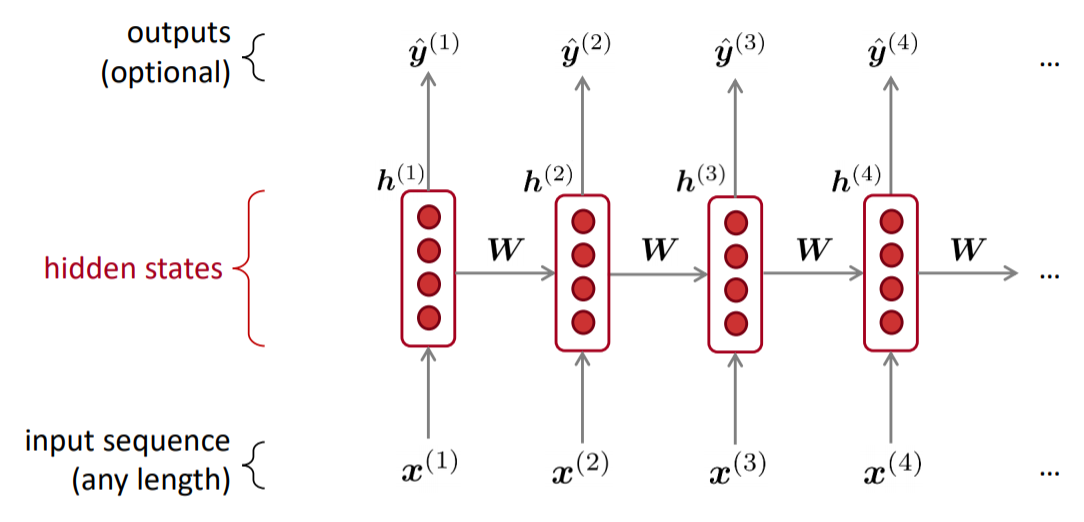
\includegraphics[width=8.0cm]{figs/RNN.png}}
	\caption{Principle of RNN}
	\label{RNN}
\end{figure}

\sidenotedcmmc{Note that for $n$-gram, increasing $n$ makes sparsity problems worse. Typically $n \le 5$.}

To process \emph{variable} length \concept{sequential input} such as text, \concept{Recurrent Neural Network} (RNN) is introduced.
As the principle of RNN shown in Fig.~\ref{RNN}: \emph{repeat} (i.e. \concept{unfold} or unroll) the same RNN cell for each time-step but with different input and previous \concept{hidden state}.
A vanilla RNN for language modeling is:
\begin{align}
\bm{h}^{(t)} &= \sigma \left(\bm{W}_h \bm{h}^{(t-1)} + \bm{W}_x \bm{x}^{(t)} + \bm{b}_1\right) \\
\hat{\bm{y}} &= P(\bm{x}^{(t)} | \bm{x}^{(t-1)}, \cdots, \bm{x}^{(1)}) \nonumber \\
&= \texttt{softmax}(\bm{U}\bm{h}^{(t)} + \bm{b}_2) 
\end{align}
where $\sigma(\cdot)$ is the activation function, and $\bm{h}^{(0)}$ is the initial (random or zero) hidden state.
The gradient w.r.t. the weight matrix is the \emph{sum} of the gradients w.r.t each time it appears using \concept{back-propagation through time} (BPTT, just as same as normal back-prop).
And the \concept{evaluation metric} for language modeling is \emph{perlexity} which is equal to the exponential of the cross-entropy losses:
\begin{align}
\text{perplexity} &= \prod_{t=1}^T \left(\frac{1}{P_{LM} (\bm{x}^{(t+1)} | \bm{x}^{(t)}, \cdots, \bm{x}^{(1)})}\right)^{\nicefrac{1}{T}} \nonumber \\
&= \exp\left(\frac{1}{T} \sum_{t=1}^T -\log \hat{\bm{y}}^{(t)}\right)
\end{align}

There are some other applications of RNN: part-of-speech tagging, named entity recognition, sentence classification, text generator, encoder module, etc.
The final feature can be the final hidden state or elemen-wise max/mean of all hidden states.
However, the \emph{vanilla} RNN has these disadvantages: (1) recurrent computation is slow (2) hard to access long-term information (\concept{long-term dependencies}) due to \emph{gradient vanish} and \emph{gradient explosion}.